Ziel dieser Arbeit ist die Konzeption einer Software, welche zu übersetzende und übersetzte Strings des Quelltext eines Movelets automatisiert verarbeitet.
\par
Im Folgenden wird das im Zuge dieser Arbeit entstandene Konzept eines Lokalisierungstools vorgestellt. Um die Verwendung des Lokalisierungstools zu ermöglichen werden zu übersetzende Strings von dem Nutzer ausgezeichnet. Zu diesem Zweck wird das \ac{ITS} und die an \textit{GNU gettext} angelehnte Auszeichnung $\_()$ verwendet. Das Lokalisierungstool nutzt die Auszeichnung um zu übersetzende von nicht zu übersetzenden Strings zu unterscheiden. In Folge dessen extrahiert das Lokalisierungstool die ausgezeichneten Strings und erstellt \ac{XLIFF} Dateien. Die extrahierten Strings werden in dem \textit{source} Element der \ac{XLIFF} Dateien gespeichert. Das \ac{XLIFF} ist ein Standard Format zu dem Austausch von Daten der Lokalisierung. 
\autocite{Schnabel.2014}
In der Konsequenz kann dieses Format ohne Kompatibilitätsprobleme von in- und/oder externen Übersetzern und deren Software übersetzt werden. Die übersetzten Strings werden in dem den \textit{source} Element zugehörigen \textit{target} Element der \ac{XLIFF} Dateien gespeichert. In Folge dessen enthält das \textit{source} Element den zu übersetzenden und das \textit{target} Element den zugehörigen übersetzten String. Aufgrund der Extraktion, stimmt der Inhalt des \textit{source} Elements mit einem ausgezeichneten String des Quelltexts des Movelets überein. Folglich wird durch das Ersetzen der ausgezeichneten Strings durch die Strings im zugehörigen \textit{target} Element eine übersetzte Version des Quelltexts erzeugt. Zu diesem Zweck werden nicht die Strings im Originalquelltext ersetzt, stattdessen wird eine Kopie erzeugt, in welcher die Ersetzung erfolgt. In der Konsequenz fungiert der Originalquelltext als Vorlage, aus welcher beliebig viele übersetzte Versionen erzeugt werden können. 
\par
Versionsverwaltung wird von diesem Lokalisierungstool selbst nicht umgesetzt, es ist jedoch empfehlenswert  Software zu der Versionsverwaltung einzusetzen.
\par
Zu dem Zweck des besseren Verständnis ist der Prozess des Lokalisierungstools von der Movelet Vorlage bis zu dem lokalisierten Movelet in Abbildung \ref{fig:zsm} veranschaulicht. Die rote Linie zwischen Movelet Vorlage und \ac{XLIFF} stellt die Extraktion der zu übersetzenden Strings dar. Die Linien zwischen Übersetzer und \ac{XLIFF} stellen den Vorgang der Übersetzung dar und die grüne Linie zwischen stellt das Ersetzen der zu Übersetzenden Strings in der Vorlage durch die übersetzten Strings dar.
\begin{figure}
	\centering
	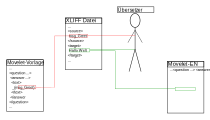
\includegraphics[width=1\textwidth]{img/zusammenfassung.pdf}
	\caption{Darstellung der Arbeitsschritte des Lokalisierungstools}
	\label{fig:zsm}
\end{figure}
